\chapter{Felhasználói dokumentáció} % User guide
\label{ch:user}

Az alkalmazás készítése során fontos szempont volt, hogy egy felhasználóbarát webáruházat hozzak létre. A webshop használata egyszerű letisztult felülettel rendelkező program olyan funkciókkal kiegészítve, amelyik megkönnyítik az átlagos vásárlók számára az oldal kezelését. A fejezet célja, hogy bemutassa az alkalmazás azon tulajdonságait, ami nem feltétlenül egyértelmű egy hétköznapi kliens számára. Ezzel is elősegítve a webalkalmazás gördülékeny felhasználását.


\section{Alkalmazás indítása} % Enumerations and lists

Egy hétköznapi felhasználó számára talán ez a legnagyobb kihívás a program használatával kapcsolatban. Az alkalmazás indítására két módszer közül választhatunk, melyek a következőek:

\begin{compactenum}
	\item Megnyitni böngésző segítségével a weboldalt. 2.1.1. fejezet
	\item Megnyitni localhostról a projektet. 2.1.2 fejezet
\end{compactenum}

\bigskip
Mindkettő technikát részletes bemutatásra kerül a következő alfejezetekben.

\subsection{Alkalmazás indítás böngészőből}
Az első és legkönnyebben alkalmazható stratégia, hogy valamilyen előre telepített webböngésző (Chrome, Firefox, Opera..stb.) segítségével megnyitjuk az előre Amazon (AWS) szerverére telepített weboldalt. A felület ezen az URL-en (rövidítés feloldása: Uniform Resource Locator) érhető el: http://webbeauty.us-east-2.elasticbeanstalk.com

\subsection{Alklamazás indítása saját gépről}
Az előző  módszert azért neveztem könnyebben alkalmazhatónk, mert ha saját gépről szeretnénk indítani az alkalmazás nem csak le kell klónoznunk azt Github segítségével, hanem több különböző szoftvert kell telepítenünk mielőtt eltudnánk indítani magát a projektet. Magához a program fordításához szükségünk lesz a Node.js szoftverre, amely letölthető ingyenesen a nodejs.org eredeti honlapjáról. Továbbá még elengedhetetlen a gépünkről az Angular CLI. Ez egy parancssori interfész az Angular szoftverhez. Mivel a kód futtatásához szükségünk van rengetek eszközre, amely lefordítja és optimalizálja a kódot. A CLI ezt biztosítja a projekt számára. A kód fordításához szükségük lesz egy integrált fejlesztői környezetre. Én személy szerint a Visual Studio Code(rövidítve VS Code) nyílt forráskódú kódszerkesztőjét használtam az alkalmazás elkészítése során, így ezt fogom bemutatni. A következő felsorolásban összefoglalom azokat a lépéseket, amik segítségével eljutunk a program saját gépről való indítását. 

\begin{enumerate}
	\item\label{step:first} https://nodejs.org-ról töltsük le és telepítsük a számítógépre megfelelő .exe kiterjesztésű fájlt.
	\item https://github.com/magyardor/szakdolgozat2021 webcímen elérhető GitHub repository-t klónozzuk le az eszközünkre
	\item töltsük le, és telepítsük a Visual Studio Code nevezetű programot a https://code.visualstudio.com címről.
	\item nyissuk meg a VS code alkalmazást és installáljuk a következő bővítményeket: Angular Essentials, Material Icon Theme
	\item a VS code segítségével töltsük be a leklónozott projekt mappáját, és nyissuk meg egy új terminált
	\item a terminálba lépjünk be a szakdolgozat nevezetű mappájába és futtassuk le a következő parancssort: npm install -g @angular/cli
	\item ha ez sikeresen megtörtént akkor futtassuk le az npm i parancssort, melynek segítségével letöltődnek azok a szükséges fájlok, amik nem szerepelnek az Angular CLI interfészben, de használatban vannak 
	\item mielőtt elindítanánk az alkalmazást be kell lépnünk a projekthez tartozó MongoDB adatbázisba és hozzá kell adnunk a hálózati hozzáférés nevezetű menüpont alatt a gépünk IP címét, különben nem tud csatlakozni a szerveroldalunk az alkalmazás által megjelenítendő adatokhoz
	\item a meglévő terminálunk mellé nyissunk meg egy újat és futtassuk le az egyikbe az npm run start a másikba az npm run start:server parancsokat, az előbbi a kliensoldalt, míg az utóbbi a szerveroldali kódokat futtatja és fordítja le
	\item ha sikeresen lefordult a kód, akkor a böngésző URL helyére a localhost:4200 címet begépelve megkapjuk a webáruház oldalát
\end{enumerate}


\section{Alkalmazás kezelése}
Az alkalmazás felületét két részre bonthatjuk. Az első rész maga a webáruház, amin a vásárlók megtekinthetik a termékeket és megrendelhetik őket, továbbá megnézhetik az üzemeltető által közzétett híreket, ezen felül különböző forrásokból információkat érhetnek el a vásárlással kapcsolatban. A második rész az üzemeltető által karbantartott adminisztrációs oldal. Ennek a felület használatához hitelesítés szükséges, ezzel is védve a vásárlók és a webáruház adatait. Az admin felületen lehetőség van ezen adatok kezelésére, szerkesztésére. 

\subsection{Webshop felület kezelése}
A webáruház kezelése igen egyszerű az átlagos felhasználók számára. Számos funkcióval rendelkezik az alkalmazás, amelyek elősegítik, hogy egy letisztult, felhasználóbarát programot használjanak a vásárlók.
Az áruház szerkezeti felépítése három fő részből áll:
\begin{description}
	\item[Menüsor] vagy más néven a toolbar. A \ref{fig.exemple-1}-es ábrán a webáruház főoldalának egy részét láthatjuk. A képen tetején található az alkalmazás webshopjához tartozó vezérlő felület, ami a programban toolbar néven található meg. A vezérlő felület bal oldalán látható különböző menüpontok, amelyek segítségével navigálhatunk a differens oldalak között. A jobb oldalán pedig különböző funkciókkal bíró ikonokat és az oldal logóját. Az első ilyen ikon a nyelvválasztó, aminek a segítségével megváltoztathatjuk az oldal nyelvezetét. Jelenleg az angol és a magyar nyelv közül lehet választani. A mellette lévő bevásárló kocsit ábrázoló ikon segítségével érhető el a felület kosár funkciója, ami tartalmazza az eddig hozzáadott termékeket. A kosárban szereplő termékek számáról egy előzetes információt kaphatunk a felette lévő jelvény számból.
	\begin{figure}[H]
		\centering
		
\includegraphics[width=1.0\textwidth,height=250px]{images/webshop_home.png}
		\caption{Az alkalmazás megjelenése}
		\label{fig.exemple-1}
	\end{figure}
	\item[A webáruház tartalma], amit szakmai nyelven body-nak nevezünk. Ez a menüsor alatt található meg, amit a fentebb kifejtett vezérlő felület segítségével különböző oldalak tartalmi részét jeleníthetjük meg. Példaként \ref{fig.example-2}-es ábra a és b részén láthatunk.
	\begin{figure}[H]
		\centering
		\subcaptionbox{Termékek oldala}{
			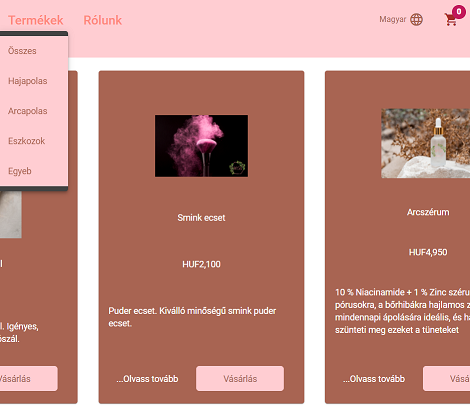
\includegraphics[width=0.45\linewidth]{images/products_page.png}}
		\hspace{5pt}
		\subcaptionbox{Hírek oldal}{
			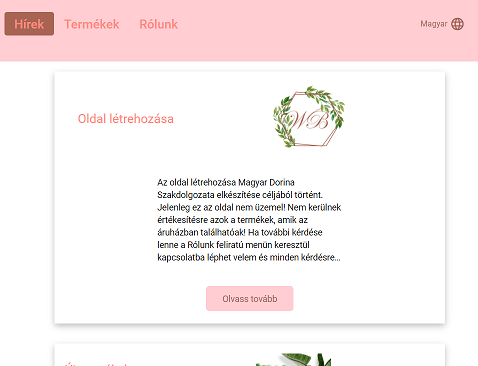
\includegraphics[width=0.45\linewidth]{images/news_page.png}}
		\caption{Webáruház tartalmi része}
		\label{fig.example-2}
	\end{figure}
	
	\item[Lábrész] vagy ahogy a programban található footer néven. A \ref{fig.exemple-3}-as képen ez a felület látható. Itt olyan oldalak linkjei jelennek meg, amik tartalmazzák a vásárlókra és az oldalra vonatkozó fogyasztóvédelmi törvényeket és általános tájékoztatókat.
	 \begin{figure}[H]
	 	\centering
	 	
\includegraphics[width=1.0\textwidth,height=120px]{images/footer.png}
	 	\caption{Az oldal lábrésze}
	 	\label{fig.exemple-3}
	 \end{figure}
	\item[Chatbot] funkció a \ref{fig.exemple-1}-es ábra legalján található zöld gomb segítségével érhető el, aminek a bemutatását a 2.3.1-es Vásárlással kapcsolatos információk alfejezetben kívánok kifejteni.
	\item[Alert üzenet] olyan információs felület, amik a felhasználó számára értesítést küld egy-egy feladat befejezésével kapcsolatban. Ilyen üzenetek lehetnek például ha nem sikerül a betöltött űrlap feldolgozása. Mint ahogy azt a \ref{fig.exemple-4}-es ábráján is láthatjuk.
	\begin{figure}[H]
		\centering
		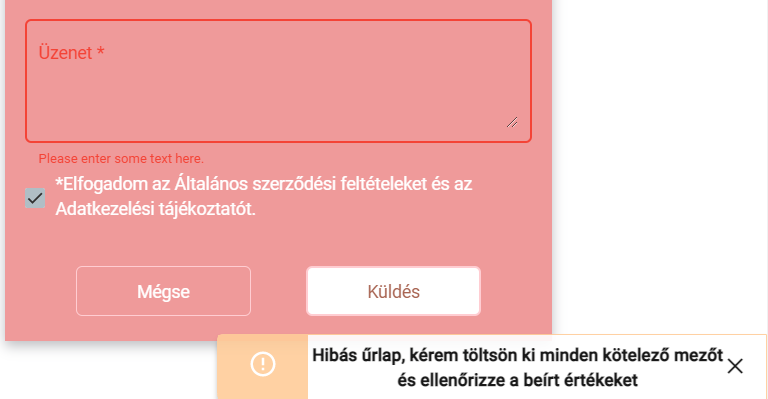
\includegraphics[width=1.0\textwidth,height=250px]{images/alert_message.png}
		\caption{Alert üzenet}
		\label{fig.exemple-4}
	\end{figure}
\end{description}


\subsection{Adminisztrációs felület kezelése}
Az oldal eléréséhez szükség van a helyesen begépelt URL megadására a böngészőnkön keresztül, ami 

\begin{compactitem}
	\item localhost esetén: http://localhost:4200/amdin/login
	\item AWS szerverre telepített weboldal esetén: http://webeauty.us-east-2.elasticbeanstall.com/admin/login
\end{compactitem}

Ha helytelenül gépeljük be a megadott webcímet, akkor az alkalmazás visszanavigál minket az oldal kezdőlapjára, viszont ha sikeresen begépeltül az adminisztrációs felület eléréséhez szükséges URL, akkor a \ref{fig.exemple-5}-ös ábrán látott oldalt láthatjuk.
	\begin{figure}[H]
	\centering
	
\includegraphics[width=1.0\textwidth,height=220px]{images/bejelentkezes.png}
	\caption{Bejelentkezési oldal}
	\label{fig.exemple-5}
\end{figure}
Az adminisztrációs felület kezeléséhez szükségünk van az oldalt védő autentikáció feloldásához. Ez azt jelenti, hogy először be kell lépnünk a fejlesztő által megadott vagy az üzemeltető által hozzáadott emailcím és jelszó párossal az előbb emlegetett címek valamelyikén. Sikeres bejelentkezéssel az oldal átnavigálásra kerül az admin felületre. Ez az oldal két főrészből áll: a vezérlési és maga a tartalmi részéből.
\begin{description}
	\item[Navigációs]felület, aminek segítségével jeleníthetjük meg az alkalmazás tartalmi részét. A \ref{fig.exemple-6}-os képen ez a navigációs rész a baloldalon található. Az admin felületen képesek vagyunk új termékeket vagy híreket hozzáadni és a meglévőket lista formájában megtekinteni. Továbbá a fentebbiekben már említett kapcsolat felvétel céljából a felhasználó által elküldött üzeneteket is kilistázásra kerülnek az oldalon. Az alkalmazáson belül lehetőségünk van új felhasználói fiókot hozzáadni, viszont ezeket a fiókokat adatvédelmi okokból nem megtekinthetőek és nem törölhetőek, csak adatbázis szinten. Ezen felül lehetőség van a bejelentkezett fiókot kijelentkeztetni, így visszalépve bejelentkezés hiányában nem tekinthetjük meg újból ezt a felület részt.
	\begin{figure}[H]
		\centering
		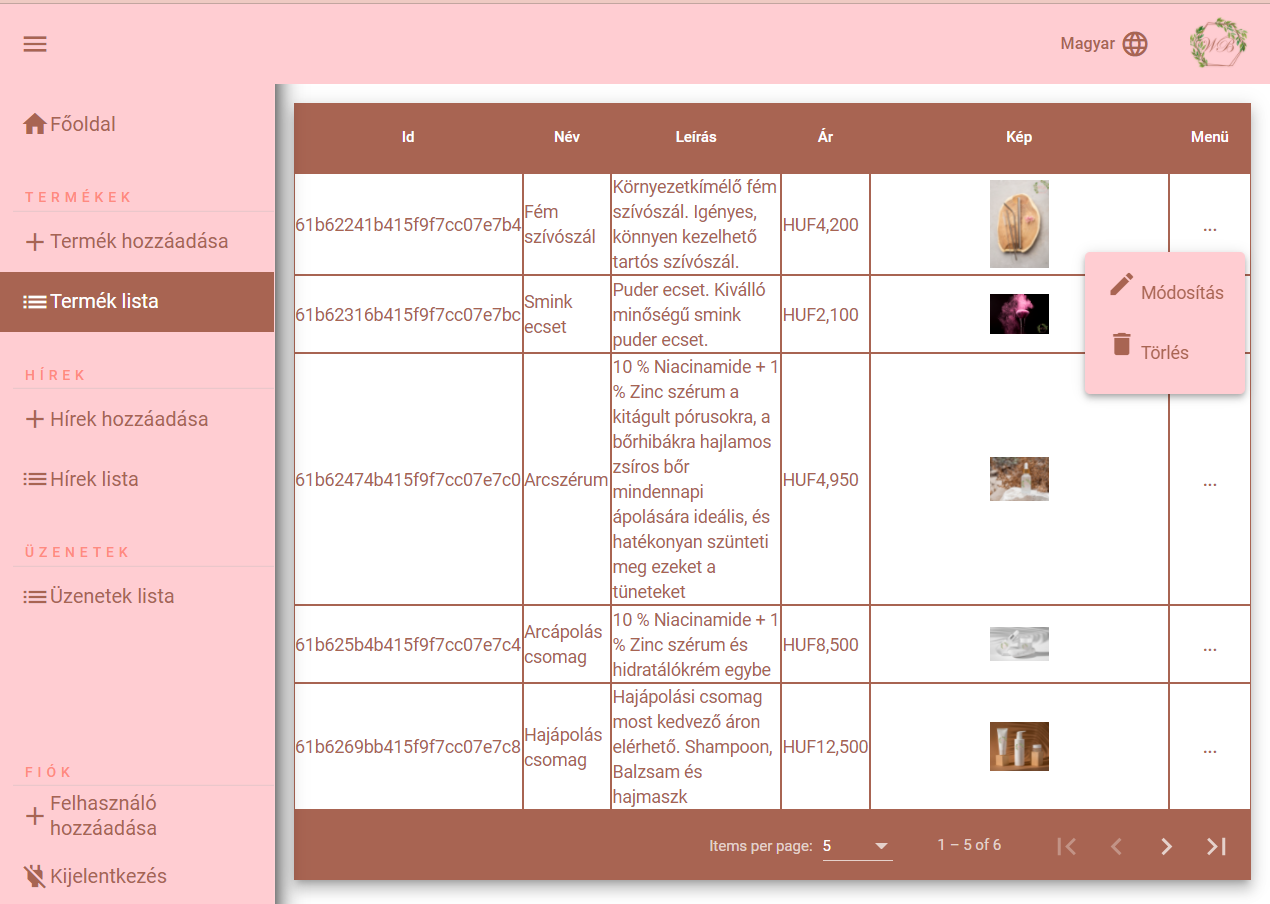
\includegraphics[width=1.0\textwidth,height=300px]{images/admin.png}
		\caption{Adminisztrációs felület megjelenése}
		\label{fig.exemple-6}
	\end{figure}
	\item[Tartalmi]rész például a \ref{fig.exemple-6}-os ábra jobboldalán látott táblázat, ami a  termékek listáját tartalmazza. Az oldal ezen részén lehetőségünk van az adatok módosítására, törlésére vagy a fentebb említett termék hozzáadására a megjelenő form kitöltésével.
\end{description}

\section{Rendelési folyamat}
A rendelés folyamata hasonlóan zajlik, mint a legtöbb webáruháznak a rendelése történik. A kiválasztott termékek bekerülnek a kosárba és személyes adatok megadásával és vásárlás befejezésével elküldésre kerül az oldal üzemeltető számára, aki előkészíti azt. A következő két alfejezetben bemutatom egy példán keresztül hogyan is kerül egy rendelés leadását a termék kiválasztásától kezdve és milyen feltételei, információ vonzatai vannak a webáruházon történő vásárlásnak.

\subsection{Rendelés leadása}
A rendelés leadásához először is szükséges, hogy valami bekerüljön a bevásárlókosár tartalmába. Termék kosárba helyezésére két lehetőségünk van. Az első, hogy ha a termékek listájánál a kiválasztott termék kártyáján a vásárlás gombra kattintunk, mint ahogy a \ref{fig.exemple-7}-es ábrán is megfigyelhető.
\begin{figure}[H]
	\centering
	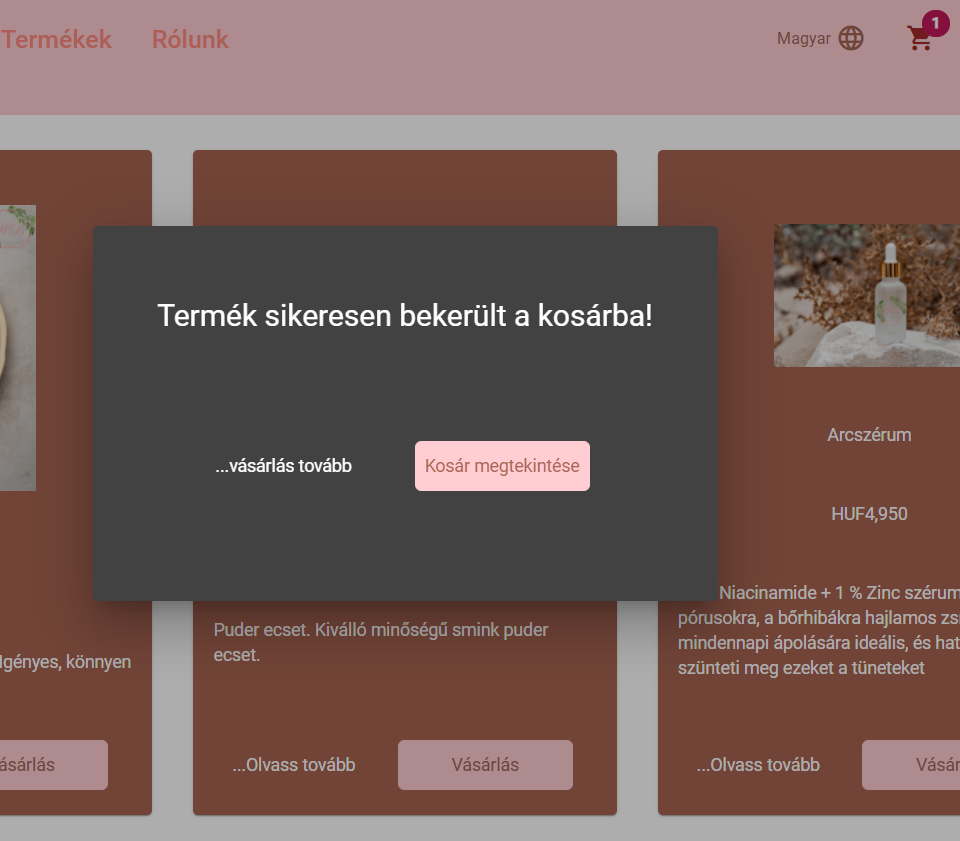
\includegraphics[width=1.0\textwidth,height=360px]{images/termek_vasarlas_1.png}
	\caption{Termék vásárlása első példa}
	\label{fig.exemple-7}
\end{figure}

A második lehetőségünk az áru bevásárlókocsiba helyezésére, hogy a kiválasztott termék profil oldalán kattintunk a vásárlás gombra. A különbség a két alternatíva között, hogy a második hozzáadás során megadhatjuk a vásárolandó áru számát. Ahogy azt a \ref{fig.exemple-8}-as második kép példáján is láthatjuk.
\begin{figure}[H]
	\centering
	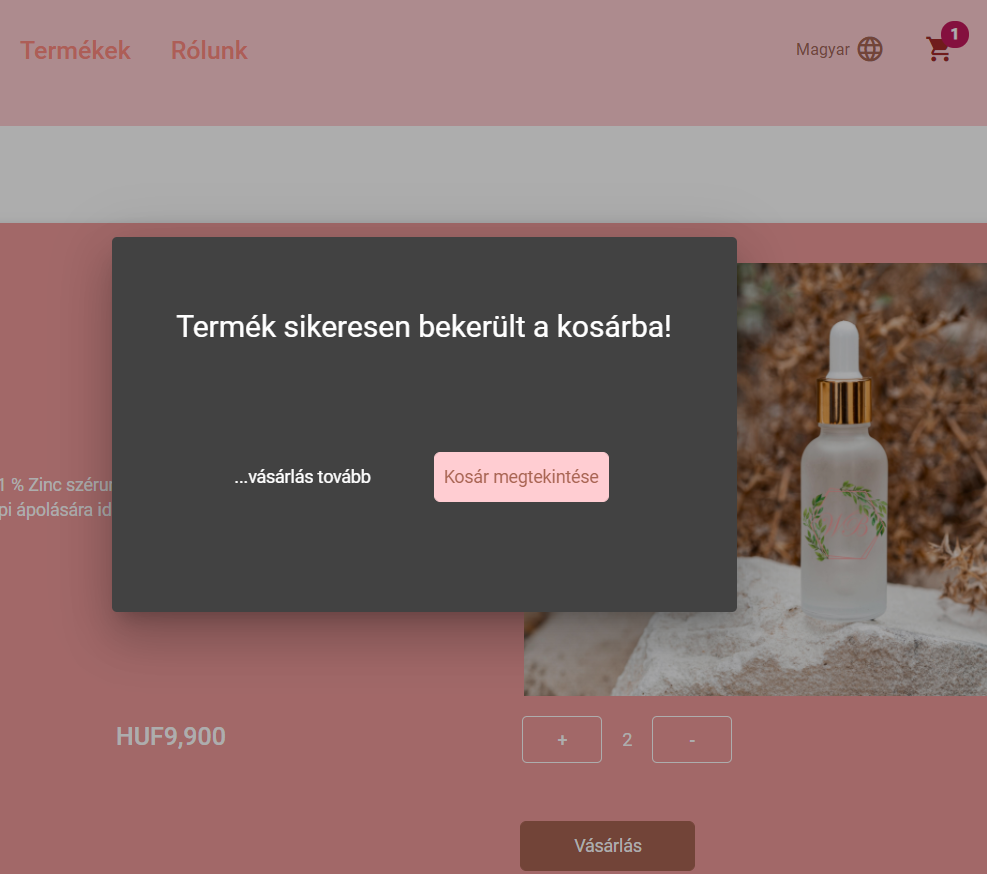
\includegraphics[width=1.0\textwidth,height=350px]{images/termek_vasarlas_2.png}
	\caption{Termék vásárlása második példa}
	\label{fig.exemple-8}
\end{figure}

Ha a kiválasztott termékek a kosárba kerültek, azokat megtekinthetjük úgy, hogy ha a \ref{fig.exemple-7}-es és a \ref{fig.exemple-8}-as ábrákon is látott Kosár megtekintése gombot kiválasztjuk, vagy ha magára a bevásárlókocsi ikonjára kattintunk. Mindkettő lehetőséggel átirányít a kosár oldalára, ahol láthatjuk táblázat formájában a megvásárolandó árukat. Mint azt a \ref{fig.exemple-9}-es képen is láthatjuk.
\begin{figure}[H]
	\centering
	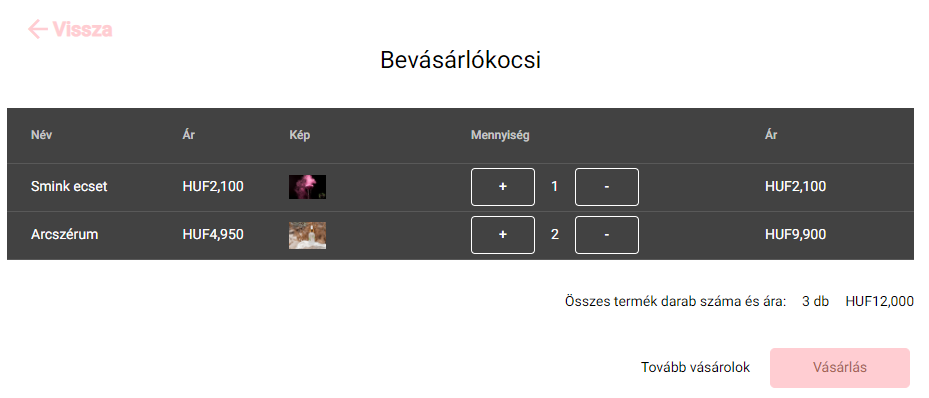
\includegraphics[width=1.0\textwidth,height=350px]{images/kosar.png}
	\caption{Bevárásló kosár}
	\label{fig.exemple-9}
\end{figure}

A bevásárlókosár tartalmának módosításra lehetőségünk van a mennyiség oszlopában látható gombok segítségével. Ha csökkentjük vagy növeljük egy áru darab mennyiségét, akkor azok az adatok, amiket ez befolyásolja dinamikusan változnak.

\bigskip
A táblázat alatti Vásárlás gombot kiválasztva az oldal átnavigál a fizetési felületre. Az alábbi \ref{fig.exemple-10}-es képeken látható, hogy ezen a felületen négy stepper button magyarul lépegető gomb található. Minden lépegetőnek külön funkciója van, amit a nevével azonosíthatunk.
\begin{figure}[H]
	\centering
	\subcaptionbox{Első stepper button}{
		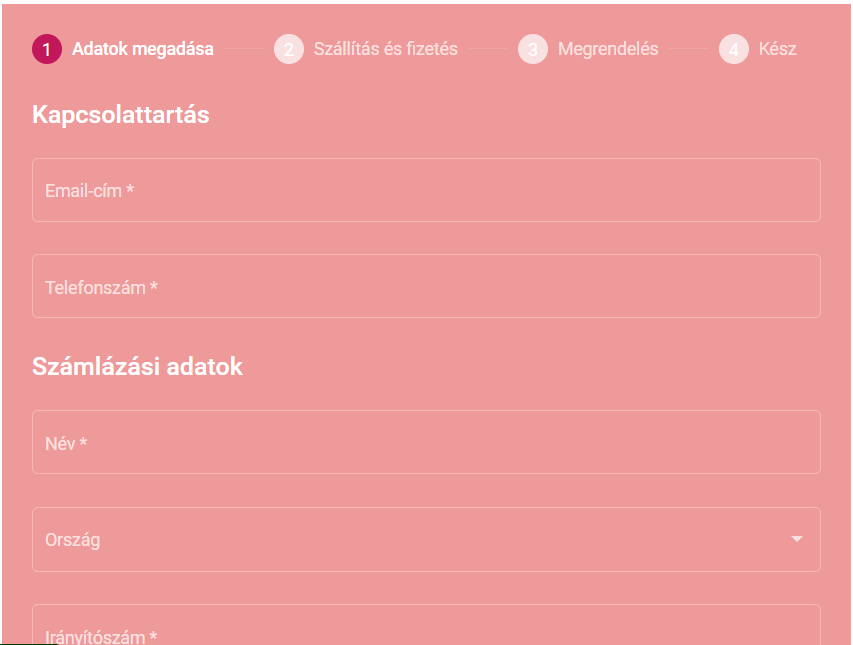
\includegraphics[width=0.45\linewidth]{images/fizetes_1.png}}
	\hspace{5pt}
	\subcaptionbox{Második stepper button}{
		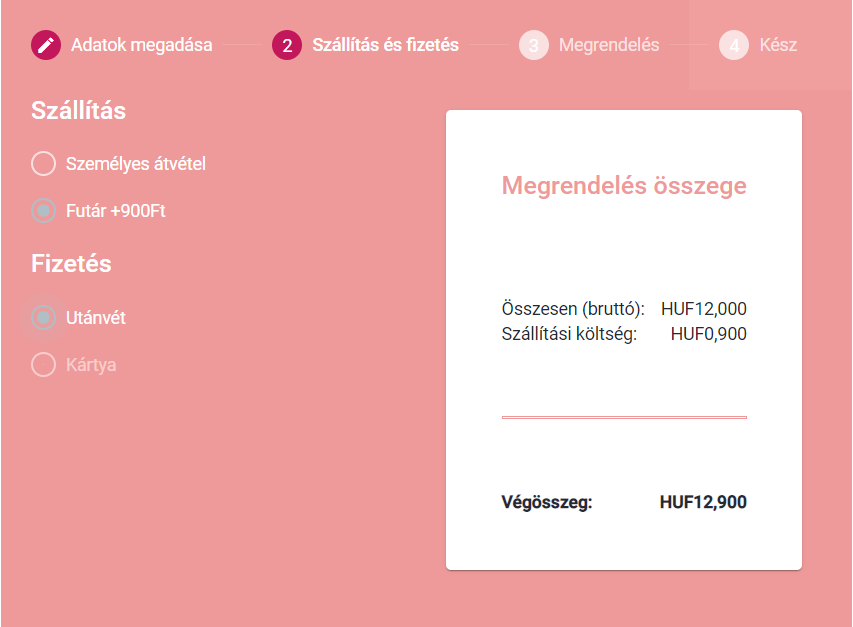
\includegraphics[width=0.45\linewidth]{images/fizetes_2.png}}
	\caption{Fizetési felület}
	\label{fig.exemple-10}
\end{figure}

Az első ilyen gombon adhatóak meg a szállítás és számlázási adatokkal kapcsolatos űrlap, aminek a helyes kitöltésével léphetünk a következő lépésre. A második stepper gombon a szállítással és fizetéssel kapcsolatos információkat adhatjuk meg. A további lépegetőkön egy összefoglalót és visszajelzést kapunk a leadott rendeléssel kapcsolatban.

\subsection{Vásárlással kapcsolatos információk}
A vásárlással kapcsolatban 